% 投稿主文。实验数值由 generated/*_macros.tex 自动注入。
\section{引言}
\label{sec:intro}

路径--速度解耦（Path--Velocity Decomposition, PVD）以路径 QP 和速度 QP 的顺序求解换取了稳定的实时性能，已成为结构化道路规划的重要工程范式\citep{kant1986pvd,fan2018baidu,apollo2024,zhou2021pathqp,zhou2021dliaps}。然而，当多个障碍物同时产生横向绕行和纵向让行需求时，传统接口只把一条确定路径传给速度阶段：路径侧过早固定“从哪边走”，速度侧再决定“何时通过”。这种单向信息流会遗漏两类关键组合：其一，多障碍物之间可能存在若干可行的空间同伦带，逐障碍物贪心选向只保留其中一个；其二，同一空间路径可能对应先通过、后通过或多个冲突间的混合时序，而单侧停止边界无法表达这些离散时序关系。

现有研究主要沿两条路线处理这一问题。联合时空规划在 $(s,l,t)$ 或更高维状态空间内同步搜索与优化\citep{morsali2021svm,hu2023_hybrid_astar_slt,micheli2023nmpc,han2024efficient,guo2024joint,hu2025_dp_nmpc}，能够直接表达空间--时间耦合，但通常需要替换成熟的路径--速度求解链。另一类工作通过迭代、候选配对或安全走廊协调两个子问题\citep{chen2019em,cheng2022gp,zhang2023_dp_rcg,yoon2024stcorridor,frenetcorridor2025,tariq2026enveloping}，保留了更多工程结构，却仍面临离散同伦选择与连续优化之间的接口问题。尤其在窄路、多障碍物交织和预测含噪场景中，如何以有限候选覆盖关键同伦类，并让选定同伦转化为两个 QP 可直接使用的线性约束，仍缺少一套统一方法。

从离散决策角度看，格点、混合 A* 与混合整数方法能够表达左右绕行，但候选数会随障碍物组合快速增长\citep{dolgov2010,kuwata2009rrt,mcnaughton2011lattice,kessler2023,narrowcorridor2022}；路径--速度候选配对则需要在候选覆盖率与实时性之间折中。动态行人与车辆交互研究进一步说明，横向绕行方向和纵向让行时机不能孤立决定\citep{crossingped2019,yangbo2023ped,pathspeedstructured2024}。UniAD 和 VAD 等端到端方法在统一表征中学习预测与规划\citep{hu2023uniad,jiang2023vad}，但其目标不是保留可解释、可验证的凸 QP 接口。表~\ref{tab:related}概括了本文与代表性路线的差别。

\begin{table}[htbp]
\centering
\caption{代表性规划路线与 MIKU 的结构比较}
\label{tab:related}
\small
\begin{adjustbox}{max width=\textwidth}
\begin{tabular}{lllll}
\toprule
路线 & 空间离散选择 & 多冲突时间次序 & 预测误差管 & 保留路径/速度 QP\\
\midrule
Apollo EM / DL-IAPS\citep{fan2018baidu,zhou2021dliaps} & 启发式 & ST 决策 & 固定缓冲 & 是\\
联合网格/NMPC\citep{hu2023_hybrid_astar_slt,guo2024joint} & 联合搜索 & 联合搜索 & 方法相关 & 否\\
候选配对/迭代\citep{cheng2022gp,zhang2023_dp_rcg} & 有限候选 & 迭代协调 & 方法相关 & 部分\\
时空安全走廊\citep{yoon2024stcorridor,frenetcorridor2025} & 走廊拓扑 & 显式时间域 & 方法相关 & 否\\
MIKU & $k+1$ 连续分割与 Top-K & 因果时间同伦图 & 有界增长管 & 是\\
\bottomrule
\end{tabular}
\end{adjustbox}
\end{table}

本文提出 MIKU（Multi-obstacle Interaction-aware Kinematic-constraint Unification），即面向解耦路径--速度规划的交互感知时空同伦走廊。其核心思想不是把动态障碍物简单投影到路径边界，而是先在鲁棒预测占据上构造有限的空间与时间同伦候选，再将选定同伦编译为路径 QP 和速度 QP 的盒约束。由此，离散层负责回答“从哪里、何时通过”，连续层仍由成熟凸优化器生成平滑轨迹。

本文的主要贡献如下：
\begin{enumerate}[leftmargin=2em]
  \item 提出一套与 Apollo 解耦规划链兼容的时空同伦走廊框架。该框架把鲁棒动态占据、Top-K 空间同伦、多冲突时序同伦和双向 ST 约束组织为统一的候选--验证闭环，无需替换原路径 QP 与速度 QP。
  \item 建立多障碍物连续分割性质。对含 $k$ 个障碍物的横向冲突组，证明 $2^k$ 个左右绕行组合的最优解可由 $k+1$ 个连续通行带覆盖，并据此构造精确最大间隙扫描与 Top-K 空间候选。
  \item 提出多冲突时序同伦图与双向 ST 走廊。通过先通过下界、后通过上界及其组合显式编码通行次序，并使用因果可达性剪枝和候选回退保持速度 QP 的可行性。
  \item 构造有界预测误差下的鲁棒占据管以及按需路径--速度交替细化。固定同伦后，新增约束保持线性，两个子问题仍为凸 QP；滚动规划进一步利用语义同伦标签和先行承诺抑制周期切换。
  \item 在 7 类、共 \RandCaseCount 个配对随机场景及 \ClosedCaseCount 个滚动场景中完成系统验证。MIKU 相对时间盲 B0 将无碰撞到达率提高 \RandAllMikuVsBZeroSuccessDiff 个百分点，碰撞率由 \RandAllBZeroCollisionPct\% 降至 \RandAllMikuCollisionPct\%；随机消融进一步分离了核心模块的贡献。
\end{enumerate}

\section{问题描述与形式化}
\label{sec:problem}

在 Frenet 坐标系中，规划轨迹写为 $\xi(t)=(s(t),l(s(t)))$。道路物理边界为 $[b^-_{\rm road}(s),b^+_{\rm road}(s)]$，自车宽度为 $W_e$，则自车中心的道路可行域为
\begin{equation}
 \mathcal B(s)=\left[b^-_{\rm road}(s)+\frac{W_e}{2}+d_{\rm road},\;
 b^+_{\rm road}(s)-\frac{W_e}{2}-d_{\rm road}\right].
 \label{eq:center-road}
\end{equation}
障碍物 $i$ 的预测占据为 $O_i(t)=[s_i^-(t),s_i^+(t)]\times[l_i^-(t),l_i^+(t)]$。路径 QP 在离散站点 $s_m$ 上优化 $l_m$，速度 QP 在离散时刻 $t_j$ 上优化 $s_j$。标准解耦接口可概括为
\begin{equation}
 l^*(s)=\arg\min_{l\in\mathcal F_l}J_l(l),\qquad
 s^*(t)=\arg\min_{s\in\mathcal F_s(l^*)}J_s(s),
 \label{eq:pvd}
\end{equation}
其中 $\mathcal F_s$ 依赖已经固定的路径。若路径阶段只保留单个横向选向，速度阶段便无法回退到另一条空间同伦；若 ST 映射只生成“障碍物前方停车”的上界，也无法表达在安全时间窗内先行通过。因此，本文把规划目标重述为：在保留式\eqref{eq:pvd}两个凸子问题的条件下，从障碍物的鲁棒时空占据中选取一对离散同伦标签
\begin{equation}
 h=(h_l,h_t)\in\mathcal H_l\times\mathcal H_t,
\end{equation}
并将其转换为横向走廊 $\mathcal C_l(h_l)$ 与纵向--时间走廊 $\mathcal C_t(h_t\mid l)$，使最终轨迹满足
\begin{equation}
 l(s)\in\mathcal C_l(h_l),\qquad s(t)\in\mathcal C_t(h_t\mid l),
 \qquad \xi(t)\notin O_i^{\rm rob}(t),\ \forall i,t.
 \label{eq:target}
\end{equation}

这里的“同伦”指在障碍物占据不被穿越时可连续变形的绕行或通行次序类别。空间标签描述障碍物位于轨迹的左侧或右侧；时间标签描述自车相对冲突占据先通过或后通过。MIKU 在离散层搜索这些标签，在连续层优化每个标签对应的轨迹质量。

\section{MIKU 时空同伦走廊方法}
\label{sec:method}

\begin{figure}[htbp]
\centering
\begin{tikzpicture}[node distance=7mm and 8mm, every node/.style={font=\small}]
  \node[modin, text width=22mm] (pred) {预测轨迹\\自车状态};
  \node[modimp, right=of pred, text width=24mm] (tube) {威胁评估\\鲁棒占据管};
  \node[modimp, right=of tube, text width=25mm] (spatial) {连续分割\\Top-K 空间带};
  \node[modimp, below=of spatial, text width=25mm] (temporal) {因果图搜索\\时间同伦};
  \node[mod, left=of temporal, text width=24mm] (qp) {路径 QP\\速度 QP};
  \node[modout, left=of qp, text width=22mm] (traj) {可执行轨迹\\语义标签};
  \draw[flow] (pred)--(tube);
  \draw[flowimp] (tube)--(spatial);
  \draw[flowimp] (spatial)--(temporal);
  \draw[flow] (temporal)--(qp);
  \draw[flow] (qp)--(traj);
  \draw[flowimp, rounded corners] (qp.north) |- node[pos=.55,above]{到达时间细化} (tube.south);
  \draw[flow, rounded corners] (traj.south) |- node[pos=.48,below]{滚动同伦保持} (temporal.south);
\end{tikzpicture}
\caption{MIKU 与解耦路径--速度求解链的闭环关系}
\label{fig:framework}
\end{figure}

如图~\ref{fig:framework}所示，MIKU 由鲁棒占据建模、空间同伦生成、时间同伦生成、QP 验证与滚动一致性五部分组成。Apollo 的边界生成、路径 QP、ST 映射和速度 QP 被保留为连续求解骨架；本文方法改变的是候选组织、约束构造及路径--速度之间的信息传递关系。

\subsection{交互威胁度与鲁棒动态占据}

为使安全裕度同时反映碰撞紧迫性、几何重叠和场景交互，定义障碍物威胁度
\begin{equation}
 \Theta_i=\sum_{r=1}^{5}w_r f_r(i),\qquad \sum_{r=1}^{5}w_r=1,
 \label{eq:threat}
\end{equation}
其中五项分别编码 TTC、纵向重叠、相对速度、障碍物类型和局部交互密度，均归一化到 $[0,1]$。障碍物横向膨胀量写为
\begin{equation}
 \delta_i=\frac{W_e}{2}+d_0+d_\Theta\Theta_i,
 \label{eq:margin}
\end{equation}
从而把统一中心语义与场景相关安全裕度结合起来。式\eqref{eq:center-road}已经将车宽计入道路边界，式\eqref{eq:margin}只在障碍物一侧完成对应的 Minkowski 膨胀，不再重复扣除整车宽度。

对含预测误差的动态障碍物，采用随时间增长的有界误差半径
\begin{equation}
 \rho_{q,i}(t)=\rho_{q,i}^{0}+t\dot\rho_{q,i},\quad q\in\{s,l\},
\end{equation}
并构造鲁棒占据管
\begin{equation}
 O_i^{\rm rob}(t)=O_i(t)\oplus
 [-\rho_{s,i}(t),\rho_{s,i}(t)]\times[-\rho_{l,i}(t),\rho_{l,i}(t)].
 \label{eq:robust-tube}
\end{equation}
该占据管同时用于路径侧投影、ST 边界映射与规划安全验证；实验评价则始终使用未扰动真值。ST 映射不是在路径中心的单点横向值上判断相交，而是在车辆纵向 Minkowski 区间内查询整段曲线路径的横向包络，从而覆盖车辆角点与弯曲路径造成的碰撞区域。

\subsection{连续分割与 Top-K 空间同伦}

给定到达时间初值 $\tau(s)$，在站点 $s$ 查询式\eqref{eq:robust-tube}，得到障碍物中心禁行区间 $[u_i(s),v_i(s)]$。首先按纵向重叠关系把活跃障碍物划分为冲突组；对一个含 $k$ 个障碍物的组，按 $u_i$ 非降序排列为 $(1),\ldots,(k)$。定义
\begin{align}
 V_p&=\max\{l^-_{\rm road},v_{(1)},\ldots,v_{(p)}\},\\
 U_p&=\min\{l^+_{\rm road},u_{(p+1)}\},\qquad p=0,\ldots,k,
 \label{eq:gap}
\end{align}
其中空前缀和空后缀分别由道路下、上界给出。第 $p$ 个连续分割的通行带为 $[V_p,U_p]$，宽度 $g_p=U_p-V_p$。

\begin{lemma}[连续分割性质]
若一个左右绕行分配可行，则存在一个不减小中心可行带宽度的分配，使排序后的前 $p$ 个障碍物位于轨迹一侧、其余障碍物位于另一侧。
\label{lem:partition}
\end{lemma}
\begin{proof}
任取存在交错的可行分配，即存在 $a<b$，较小 $u_{(a)}$ 被分到上界侧、较大 $u_{(b)}$ 被分到下界侧。交换或消去该逆序不会收紧当前上界的最小值，也不会抬高下界的最大值。反复消除逆序后得到单一分割点 $p$，且通行带宽度不减。
\end{proof}

\begin{theorem}[最大间隙精确性]
组内全部 $2^k$ 个左右绕行分配的最大中心可行宽度等于
\begin{equation}
 g^*=\max_{p\in\{0,\ldots,k\}}(U_p-V_p).
\end{equation}
因此，经排序、前缀最大和一次扫描可在 $O(k\log k)$ 时间内得到精确最大间隙。
\label{thm:maxgap}
\end{theorem}
\begin{proof}
固定连续分割点 $p$ 后，同侧约束的交集边界恰为式\eqref{eq:gap}中的 $V_p$ 与 $U_p$，故其宽度为 $g_p$。由引理~\ref{lem:partition}，至少一个全局最优分配属于这 $k+1$ 个连续分割，结论成立。
\end{proof}

MIKU 不只保留 $g^*$ 对应的一条通行带，而是依据净宽度、参考线偏移和相邻组同伦切换代价对全部可行 $[V_p,U_p]$ 排序。每组保留 $Q$ 个通行带，将各障碍物组构造为分层有向图。动态规划在每个当前带上保留代价最低的 $K$ 条前缀；由于后续代价只通过前缀的末端带与其相关，该过程给出一阶分层图上的精确 K-best 全局空间同伦。对 $M$ 个分组，其复杂度为 $O(MKQ^2\log(KQ))$；本文取 $Q=K=3$。最大间隙定理和精确 K-best 连接共同避免了对组内左右组合及跨组路径的穷举，并为后续时间约束和 QP 可行性保留有序回退空间。

\subsection{多冲突时间同伦图与双向 ST 走廊}

对一条空间候选路径，MIKU 将与鲁棒占据管相交的区域映射为按纵向排序的冲突点 $c_r=(s_r,\mathcal I_r)$，其中 $\mathcal I_r$ 是该站点的占用时间区间集合。其补集给出安全时间窗。每个安全窗对应一个时间同伦节点：位于第一个占用区间之前时标签为 \texttt{pass-before}，位于最后一个占用区间之后时标签为 \texttt{yield-after}，夹在两个占用区间之间的窗口同时具有前一冲突的后通过约束与后一冲突的先通过约束。

相邻冲突节点之间仅在满足站点顺序和运动学因果条件时连边：
\begin{equation}
 t_b-t_a\ge \frac{s_b-s_a}{v_{\max}}.
 \label{eq:causal}
\end{equation}
图搜索以时间偏差、等待代价和同伦切换为边权，使用宽度为 8 的确定性 beam 保留排名靠前的完整时间同伦。对于选中的占用区间 $[t_i^-,t_i^+]$ 及纵向冲突范围 $[s_i^-,s_i^+]$，两类标签分别编译为
\begin{align}
 \text{pass-before:}&\quad s(t_j)\ge s_i^++\varepsilon_s, &&t_j\ge t_i^+,\label{eq:pass}\\
 \text{yield-after:}&\quad s(t_j)\le s_i^--\varepsilon_s, &&t_j<t_i^- .\label{eq:yield}
\end{align}
式\eqref{eq:pass}是先行通过所需的 ST 下界，式\eqref{eq:yield}是等待障碍物离开所需的 ST 上界。两者共同构成双向时序走廊，避免把所有动态冲突都退化为停车让行。候选按排名逐个送入速度 QP；若高排名同伦不可行，则自动验证下一候选。

\begin{proposition}[固定同伦下的凸性保持]
若原路径与速度目标为凸二次函数、动力学约束为线性约束，则固定 $(h_l,h_t)$ 后，MIKU 生成的空间带、式\eqref{eq:pass}与式\eqref{eq:yield}均为逐点线性盒约束，路径 QP 与速度 QP 的凸性不变。
\end{proposition}

\begin{proposition}[占据包含下的鲁棒安全性]
若真实障碍物占据满足 $O_i^{\rm true}(t)\subseteq O_i^{\rm rob}(t)$，且连续执行轨迹始终位于按式\eqref{eq:robust-tube}构造的时空走廊内，则执行轨迹与 $O_i^{\rm true}(t)$ 不相交。
\end{proposition}
\begin{proof}
走廊构造排除了 $O_i^{\rm rob}(t)$ 与车辆 Minkowski 足迹。真实占据是该集合的子集，故对更大集合保持不相交蕴含对真实占据不相交。
\end{proof}

\subsection{路径--速度交替细化与滚动一致性}

首轮到达时间由二阶运动学模型初始化。得到速度解 $s^{(r)}(t)$ 后，从首次到达时刻反演 $\hat\tau^{(r)}(s)$，再以
\begin{equation}
 \tau^{(r+1)}(s)=(1-\alpha)\tau^{(r)}(s)+\alpha\hat\tau^{(r)}(s),
 \qquad \alpha=0.7
 \label{eq:refine}
\end{equation}
更新动态占据查询。细化只在纯动态冲突导致首轮不可行时触发：每周期最多执行两次完整规划（初始求解与一次反馈细化），并保留已验证的最佳可行解。因此其作用是修正路径--速度时序不一致，而非无条件增加每周期计算。

滚动规划中，同一冲突的空间带和时间窗被编码为语义标签，并在相邻周期加入切换惩罚。对于已验证的 \texttt{pass-before} 轨迹，在车辆越过冲突区之前保持该先行承诺，防止临近冲突点时因观测更新突然切换为后通过。该机制把单周期同伦选择扩展为跨周期一致的交互决策。

\begin{algorithm}[htbp]
\small
\caption{MIKU 时空同伦走廊规划}
\label{alg:miku}
\KwIn{自车状态、道路边界、障碍物预测与上一周期语义标签}
\KwOut{路径 $l(s)$、速度 $s(t)$ 与同伦标签 $h$}
构造威胁相关安全裕度与鲁棒动态占据管；初始化 $\tau^{(0)}(s)$\;
\For{$r=0,1$}{
  扫描线分组；由 $k+1$ 个连续分割生成并连接 Top-K 空间同伦\;
  \For{按代价排序的每条空间候选}{
    求路径 QP，并用整段路径包络建立冲突点与安全时间窗\;
    在因果图上生成多冲突时间同伦\;
    \For{按代价排序的每条时间候选}{
      将先/后通过标签写成双向 ST 盒约束并求速度 QP\;
      若轨迹通过鲁棒占据验证，则加入可行解集\;
    }
  }
  若已有可行解或无需动态细化，则退出；否则按式\eqref{eq:refine}更新时间索引\;
}
选择代价最小的可行解；在滚动周期中保持语义同伦与先行承诺\;
\end{algorithm}

对单个含 $k$ 个障碍物的横向组，候选生成复杂度为 $O(k\log k)$。全局 K-best 空间连接的复杂度如上为 $O(MKQ^2\log(KQ))$。若时间图含 $R$ 个冲突点、每点至多 $W$ 个窗口、beam 宽度为 $B$，则单条空间候选的时间协调复杂度为 $O(RBW)$。本文取 $K=Q=3,B=8$，并对每条空间候选最多验证 3 条排名靠前的时间候选，因而离散协调相对障碍物数保持多项式增长。QP 次数由候选验证和按需细化决定，实际全周期耗时在第~\ref{sec:experiment}节报告。

\section{实验验证}
\label{sec:experiment}

\subsection{实验协议}

实验基于同一套 Apollo 风格路径--速度规划链比较四种方法：B0 为时间盲固定裕度与逐障碍物贪心选向；B1 加入到达时间投影，但仍使用单一空间选向；B2 采用路径--速度迭代更新到达时间；MIKU 启用鲁棒占据、差异化裕度、分组连续分割、Top-K 空间候选、时间同伦图、双向 ST 约束与按需细化。所有方法共享车辆尺寸、道路边界、预测输入、路径/速度 QP、动力学界和目标权重，从而把差异集中在时空约束组织方式上。

主实验包含行人横穿、车辆切入、停车车辆与对向车、窄路多障碍物、多动态障碍物交织、预测含噪和延迟横穿 7 类场景。每类使用从 0 开始的 \RandSeedCount 个固定随机种子，共 \RandCaseCount 个逐场景配对实例。预测含噪类对规划器输入施加定位与速度扰动，而评价使用未扰动真值。成功定义为在规划时域内无碰撞到达评价线；碰撞由自车和障碍物实体矩形的连续时序重叠判定。完整周期耗时覆盖约束构造、候选生成、路径 QP、ST 映射、速度 QP和实际触发的细化。

二元配对结果使用精确 McNemar 检验；比例差的 95\% 置信区间由 5,000 次配对 bootstrap 得到。主实验按单进程顺序执行，以避免并发对墙钟计时的污染。硬件为 Intel Core i9-14900HX，系统为 Linux 7.2.2，QP 求解器为 OSQP 1.1.1\citep{stellato2020osqp}。原始 CSV、失败样本、统计结果与文中数值宏均由实验脚本一次生成。

\subsection{主结果：可达性、安全性与实时性}

\begin{table}[htbp]
\centering
\caption{7 类随机场景总体结果（每种方法 $n=\RandCaseCount$）}
\label{tab:overall}
\small
\begin{adjustbox}{max width=\textwidth}
\begin{tabular}{lrrrrrrrr}
\toprule
方法 & 无碰撞到达(\%) & 碰撞(\%) & 停车(\%) & 最小间距(m) & jerk RMS & P50(ms) & P95(ms) & P99(ms)\\
\midrule
B0 & \RandAllBZeroSuccessPct & \RandAllBZeroCollisionPct & \RandAllBZeroStopPct & \RandAllBZeroClearance & \RandAllBZeroJerkRms & \RandAllBZeroRuntimePfifty & \RandAllBZeroRuntimePninetyfive & \RandAllBZeroRuntimePninetynine\\
B1 & \RandAllBOneSuccessPct & \RandAllBOneCollisionPct & \RandAllBOneStopPct & \RandAllBOneClearance & \RandAllBOneJerkRms & \RandAllBOneRuntimePfifty & \RandAllBOneRuntimePninetyfive & \RandAllBOneRuntimePninetynine\\
B2 & \RandAllBTwoSuccessPct & \RandAllBTwoCollisionPct & \RandAllBTwoStopPct & \RandAllBTwoClearance & \RandAllBTwoJerkRms & \RandAllBTwoRuntimePfifty & \RandAllBTwoRuntimePninetyfive & \RandAllBTwoRuntimePninetynine\\
MIKU & \RandAllMikuSuccessPct & \RandAllMikuCollisionPct & \RandAllMikuStopPct & \RandAllMikuClearance & \RandAllMikuJerkRms & \RandAllMikuRuntimePfifty & \RandAllMikuRuntimePninetyfive & \RandAllMikuRuntimePninetynine\\
\bottomrule
\end{tabular}
\end{adjustbox}
\end{table}

表~\ref{tab:overall}表明，MIKU 的无碰撞到达率达到 \RandAllMikuSuccessPct\%，B0、B1 和 B2 分别为 \RandAllBZeroSuccessPct\%、\RandAllBOneSuccessPct\% 和 \RandAllBTwoSuccessPct\%。相对 B0，MIKU 的配对提升为 \RandAllMikuVsBZeroSuccessDiff 个百分点，95\% CI [\RandAllMikuVsBZeroSuccessCiLow,\RandAllMikuVsBZeroSuccessCiHigh]，精确 McNemar $p=\RandAllMikuVsBZeroSuccessMcNemarP$。这意味着提升来自大量相同场景上的结果翻转，而非不同难度样本的非配对均值差。

安全性方面，MIKU 碰撞率为 \RandAllMikuCollisionPct\%，B0 为 \RandAllBZeroCollisionPct\%，配对差为 \RandAllMikuVsBZeroCollisionDiff 个百分点，95\% CI [\RandAllMikuVsBZeroCollisionCiLow,\RandAllMikuVsBZeroCollisionCiHigh]，McNemar $p=\RandAllMikuVsBZeroCollisionMcNemarP$。因此，通行率提升没有以增加碰撞为代价；鲁棒占据使总体碰撞率同步下降。MIKU 完整周期 P95 为 \RandAllMikuRuntimePninetyfive\,ms，保持在线规划所需的毫秒至百毫秒内求解量级，并显著低于多轮 B2 的 \RandAllBTwoRuntimePninetyfive\,ms。

\begin{figure}[htbp]
\centering
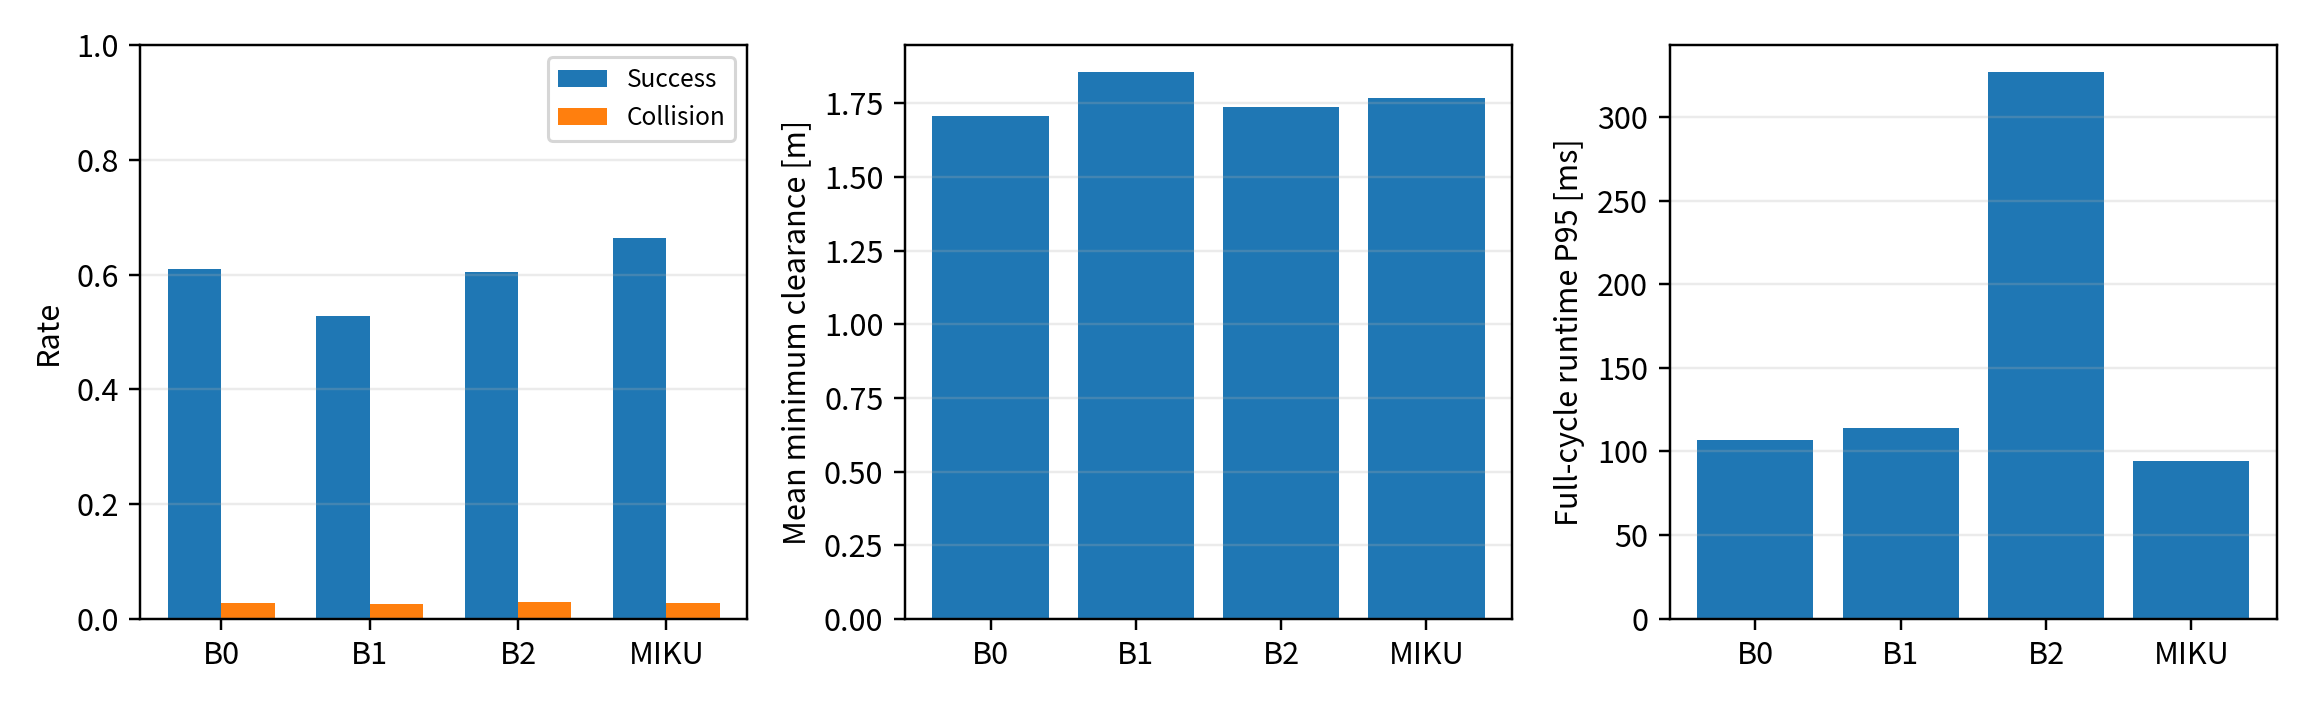
\includegraphics[width=0.96\textwidth]{generated/randomized_summary.png}
\caption{7 类配对随机场景的总体性能}
\label{fig:summary}
\end{figure}

\subsection{分场景结果}

\begin{table}[htbp]
\centering
\caption{MIKU 相对 B0 的分场景无碰撞到达率}
\label{tab:by-family}
\small
\begin{adjustbox}{max width=\textwidth}
\begin{tabular}{lrrrrr}
\toprule
场景 & B0(\%) & MIKU(\%) & 配对差(pp) & 95\% CI & McNemar $p$\\
\midrule
行人横穿 & \RandCrossingBZeroSuccessPct & \RandCrossingMikuSuccessPct & \RandCrossingMikuVsBZeroSuccessDiff & [\RandCrossingMikuVsBZeroSuccessCiLow,\RandCrossingMikuVsBZeroSuccessCiHigh] & \RandCrossingMikuVsBZeroSuccessMcNemarP\\
车辆切入 & \RandCutInBZeroSuccessPct & \RandCutInMikuSuccessPct & \RandCutInMikuVsBZeroSuccessDiff & [\RandCutInMikuVsBZeroSuccessCiLow,\RandCutInMikuVsBZeroSuccessCiHigh] & \RandCutInMikuVsBZeroSuccessMcNemarP\\
停车+对向车 & \RandParkedBZeroSuccessPct & \RandParkedMikuSuccessPct & \RandParkedMikuVsBZeroSuccessDiff & [\RandParkedMikuVsBZeroSuccessCiLow,\RandParkedMikuVsBZeroSuccessCiHigh] & \RandParkedMikuVsBZeroSuccessMcNemarP\\
窄路多障碍 & \RandNarrowBZeroSuccessPct & \RandNarrowMikuSuccessPct & \RandNarrowMikuVsBZeroSuccessDiff & [\RandNarrowMikuVsBZeroSuccessCiLow,\RandNarrowMikuVsBZeroSuccessCiHigh] & \RandNarrowMikuVsBZeroSuccessMcNemarP\\
多动态交织 & \RandInterleavedBZeroSuccessPct & \RandInterleavedMikuSuccessPct & \RandInterleavedMikuVsBZeroSuccessDiff & [\RandInterleavedMikuVsBZeroSuccessCiLow,\RandInterleavedMikuVsBZeroSuccessCiHigh] & \RandInterleavedMikuVsBZeroSuccessMcNemarP\\
预测含噪 & \RandNoiseBZeroSuccessPct & \RandNoiseMikuSuccessPct & \RandNoiseMikuVsBZeroSuccessDiff & [\RandNoiseMikuVsBZeroSuccessCiLow,\RandNoiseMikuVsBZeroSuccessCiHigh] & \RandNoiseMikuVsBZeroSuccessMcNemarP\\
延迟横穿 & \RandDelayedBZeroSuccessPct & \RandDelayedMikuSuccessPct & \RandDelayedMikuVsBZeroSuccessDiff & [\RandDelayedMikuVsBZeroSuccessCiLow,\RandDelayedMikuVsBZeroSuccessCiHigh] & \RandDelayedMikuVsBZeroSuccessMcNemarP\\
\bottomrule
\end{tabular}
\end{adjustbox}
\end{table}

MIKU 在窄路多障碍中提升 \RandNarrowMikuVsBZeroSuccessDiff 个百分点，说明连续分割与差异化裕度能够恢复被贪心边界压缩的空间通道；在延迟横穿中提升 \RandDelayedMikuVsBZeroSuccessDiff 个百分点，体现了先通过/后通过双向 ST 同伦对通行时机的表达能力。预测含噪场景的到达率提升为 \RandNoiseMikuVsBZeroSuccessDiff 个百分点，其碰撞率配对差为 \RandNoiseMikuVsBZeroCollisionDiff 个百分点，验证了鲁棒占据管的安全作用。行人横穿和多动态交织两类已接近饱和，MIKU 与 B0 保持相当成功率。

\subsection{大规模随机消融}

为避免只在少数手工构型中解释模块作用，消融实验复用主实验相同的 7 类、\RandCaseCount 个种子配对，分别关闭：A1 到达时间初始化投影，A2 障碍物分组，A3 Top-K 连续空间同伦，A4 威胁相关裕度，A5 时间同伦图，A6 鲁棒占据管，A7 交替细化。表~\ref{tab:ablation}中的差值均定义为完整 MIKU 减对应消融版本。

\begin{table}[htbp]
\centering
\caption{MIKU 组件的 \RandCaseCount 例配对随机消融}
\label{tab:ablation}
\small
\begin{adjustbox}{max width=\textwidth}
\begin{tabular}{lrrrrr}
\toprule
配置 & 到达率(\%) & 碰撞率(\%) & 完整方法增益(pp) & 95\% CI & McNemar $p$\\
\midrule
完整 MIKU & \AblMikuSuccessPct & \AblMikuCollisionPct & --- & --- & ---\\
A1 无到达时间初始化 & \AblAOneSuccessPct & \AblAOneCollisionPct & \AblMikuVsAOneSuccessDiff & [\AblMikuVsAOneSuccessCiLow,\AblMikuVsAOneSuccessCiHigh] & \AblMikuVsAOneSuccessMcNemarP\\
A2 无纵向分组 & \AblATwoSuccessPct & \AblATwoCollisionPct & \AblMikuVsATwoSuccessDiff & [\AblMikuVsATwoSuccessCiLow,\AblMikuVsATwoSuccessCiHigh] & \AblMikuVsATwoSuccessMcNemarP\\
A3 无 Top-K 空间同伦 & \AblAThreeSuccessPct & \AblAThreeCollisionPct & \AblMikuVsAThreeSuccessDiff & [\AblMikuVsAThreeSuccessCiLow,\AblMikuVsAThreeSuccessCiHigh] & \AblMikuVsAThreeSuccessMcNemarP\\
A4 无威胁相关裕度 & \AblAFourSuccessPct & \AblAFourCollisionPct & \AblMikuVsAFourSuccessDiff & [\AblMikuVsAFourSuccessCiLow,\AblMikuVsAFourSuccessCiHigh] & \AblMikuVsAFourSuccessMcNemarP\\
A5 无时间同伦图 & \AblAFiveSuccessPct & \AblAFiveCollisionPct & \AblMikuVsAFiveSuccessDiff & [\AblMikuVsAFiveSuccessCiLow,\AblMikuVsAFiveSuccessCiHigh] & \AblMikuVsAFiveSuccessMcNemarP\\
A6 无鲁棒占据管 & \AblASixSuccessPct & \AblASixCollisionPct & \AblMikuVsASixSuccessDiff & [\AblMikuVsASixSuccessCiLow,\AblMikuVsASixSuccessCiHigh] & \AblMikuVsASixSuccessMcNemarP\\
A7 无交替细化 & \AblASevenSuccessPct & \AblASevenCollisionPct & \AblMikuVsASevenSuccessDiff & [\AblMikuVsASevenSuccessCiLow,\AblMikuVsASevenSuccessCiHigh] & \AblMikuVsASevenSuccessMcNemarP\\
\bottomrule
\end{tabular}
\end{adjustbox}
\end{table}

Top-K 空间同伦和威胁相关裕度分别贡献 \AblMikuVsAThreeSuccessDiff 与 \AblMikuVsAFourSuccessDiff 个百分点，是恢复窄路空间可行性的主要来源；时间同伦图贡献 \AblMikuVsAFiveSuccessDiff 个百分点，表明动态冲突需要显式的通行次序。关闭鲁棒占据后碰撞率从 \AblMikuCollisionPct\% 增至 \AblASixCollisionPct\%，完整方法的碰撞率配对差为 \AblMikuVsASixCollisionDiff 个百分点（$p=\AblMikuVsASixCollisionMcNemarP$），直接验证了不确定性管的安全收益。交替细化带来 \AblMikuVsASevenSuccessDiff 个百分点增益，而 A1 差异未达显著，说明二阶到达时间主要提供首轮初始化，最终性能来自同伦搜索、QP 验证和反馈细化的共同作用。

\subsection{滚动规划与联合参照}

滚动实验以 0.5\,s 为执行步长循环“规划--执行--更新预测”，每类 100 个种子，共 \ClosedCaseCount 个场景。MIKU 到达率为 \ClosedMikuSuccessPct\%，B0 为 \ClosedBZeroSuccessPct\%，配对提升 \ClosedMikuVsBZeroSuccessDiff 个百分点，95\% CI [\ClosedMikuVsBZeroSuccessCiLow,\ClosedMikuVsBZeroSuccessCiHigh]，McNemar $p=\ClosedMikuVsBZeroSuccessMcNemarP$。两者碰撞率均为 \ClosedMikuCollisionPct\%。这说明语义同伦保持和先行承诺能够把单周期收益延续到连续重规划，同时没有增加碰撞。表~\ref{tab:closed-joint}中的滚动 P95 是每个场景约 20 个规划周期的累计墙钟时间，并非单周期延迟。

B3 联合参照在 $(t,s,l,v,\dot l)$ 网格上同步搜索，并与 MIKU 使用相同的威胁相关裕度和鲁棒预测管。它不使用路径--速度顺序 QP，因此用于检验解耦方法与联合候选搜索的质量--开销关系，而不是作为连续全局最优上界。

\begin{table}[htbp]
\centering
\caption{滚动规划与联合时空参照结果}
\label{tab:closed-joint}
\small
\begin{tabular}{llrrrr}
\toprule
协议 & 方法 & $n$ & 到达率(\%) & 碰撞率(\%) & P95耗时(ms)\\
\midrule
滚动规划 & B0 & \ClosedCaseCount & \ClosedBZeroSuccessPct & \ClosedBZeroCollisionPct & \ClosedBZeroRuntimePninetyfive\\
滚动规划 & MIKU & \ClosedCaseCount & \ClosedMikuSuccessPct & \ClosedMikuCollisionPct & \ClosedMikuRuntimePninetyfive\\
联合参照 & B3 & \JointCaseCount & \JointBThreeSuccessPct & \JointBThreeCollisionPct & \JointBThreeRuntimePninetyfive\\
联合参照 & MIKU & \JointCaseCount & \JointMikuSuccessPct & \JointMikuCollisionPct & \JointMikuRuntimePninetyfive\\
\bottomrule
\end{tabular}
\end{table}

联合参照中，MIKU 与 B3 的到达率差为 \JointMikuVsBThreeSuccessDiff 个百分点，95\% CI [\JointMikuVsBThreeSuccessCiLow,\JointMikuVsBThreeSuccessCiHigh]，McNemar $p=\JointMikuVsBThreeSuccessMcNemarP$；两者在当前样本中的到达率无显著差异。B3 的 P95 为 \JointBThreeRuntimePninetyfive\,ms，MIKU 为 \JointMikuRuntimePninetyfive\,ms。该对照显示，MIKU 以两个凸 QP 和有限同伦候选取得了与联合网格参照相当的可达性，同时将计算开销降低两个数量级。B3 在成功样本上的通行效率更高，说明联合搜索在时间最优性上仍有优势。

\subsection{灵敏度与适用范围}

对五项威胁权重同时施加 $\pm\SensPerturbPct\%$ 扰动并重新归一，安全裕度最大相对偏差为 \SensWorstRelDev\%；4 个代表性场景各运行 \SensTrajectoryTrialCount 条完整轨迹，共 80 条均保持成功，最大横向轨迹偏差为 0.011\,m。结果表明，方法对权重的局部变化稳定，核心收益不依赖单个精确调参点。

本文实验覆盖规划器在环的结构化道路与有界预测扰动，尚未包含真实感知误检、复杂路口规则和车辆执行器误差。该范围不影响本文对同伦候选、凸性保持和配对仿真结果的验证，也明确了下一阶段实车与概率预测实验的接口。


\section{结论}
\label{sec:conclusion}

本文提出 MIKU 时空同伦走廊，将多障碍物空间绕行、动态冲突通行次序和预测不确定性统一到现有路径--速度解耦求解链中。连续分割定理把组内 $2^k$ 个方向组合化为 $k+1$ 个通行带；多冲突时间图将先通过、后通过及其组合编译为双向 ST 约束；Top-K 回退、按需交替细化和滚动语义保持共同形成从候选生成到可执行轨迹的完整闭环。固定同伦后两个连续子问题仍为凸 QP，因此方法在扩展决策能力的同时保留了解耦规划的求解结构。

在 \RandCaseCount 个配对随机场景中，MIKU 获得 \RandAllMikuSuccessPct\% 的无碰撞到达率，相对 B0 提升 \RandAllMikuVsBZeroSuccessDiff 个百分点；碰撞率由 B0 的 \RandAllBZeroCollisionPct\% 降至 \RandAllMikuCollisionPct\%。在 \ClosedCaseCount 个滚动场景中，到达率进一步保持 \ClosedMikuVsBZeroSuccessDiff 个百分点的配对优势。大规模随机消融表明，Top-K 空间同伦、交互裕度和时间同伦图分别贡献了 \AblMikuVsAThreeSuccessDiff、\AblMikuVsAFourSuccessDiff 和 \AblMikuVsAFiveSuccessDiff 个百分点的到达率。上述结果验证了 MIKU 对密集空间约束、动态通行次序和预测偏差的协同处理能力。

当前验证集中于结构化道路的规划器在环场景。后续将把鲁棒占据半径由标定常数扩展为数据驱动的概率预测置信域，并在更复杂道路拓扑、实车感知输出及控制执行闭环中验证方法。
